\documentclass[12pt,a4paper]{article}
\usepackage{amsmath}
\usepackage{mathrsfs}
\usepackage{cancel}
\usepackage{color}
\usepackage{circuitikz}
\usepackage{url}

\begin{document} 
\section{The monodomain model} \label{The monodomain model}
The monodomain equations are given by 
\begin{eqnarray} \label{eq:a}
\frac{\partial \mathbf{s}}{\partial t}= \mathbf{F}(\mathbf{s},v), \qquad \mathbf{x} \in H, \\
\frac{\partial v}{\partial t} + I_{ion}(v,\mathbf{s}) =\nabla \label{eq:b} \cdot(\mathbf{M}\nabla v) + I_s,\qquad \mathbf{x} \in H, \\ \label{eq:c}
\mathbf{n}\cdot (\mathbf{M}\nabla v)=0, \qquad \mathbf{x} \in \delta H,
\end{eqnarray}
with $v(\mathbf{x},t)$ the transmembrane potential (in mV), $H$ the domain, $\delta H$ the boundary of $H$, $\mathbf{n}$ the outward pointing normal of the boundary, and with $I_s$ the prescribed input current (in mV/ms) and $I_{ion}$ the ionic current across the membrane (in mV/ms), both scaled by the cell membrane capacitance (in $\mu$F/(mm$^2$)). 
Equation \eqref{eq:a} is a system of ODE's that models the membrane dynamics. There exist many different cell membrane dynamics models with varying degrees of complexity that can be used to specify $I_{ion}$, $\mathbf{F}(\mathbf{s},v)$ and the state variables $\mathbf{s}(\mathbf{x},t)$, see the CellML repository\footnote{\url{models.cellml.org/electrophysiology}} for an overview of different types of models. \\ Finally, $\mathbf{M}$ is a conductivity tensor (in mm$^2$/ms), that satisfies 
\begin{equation}
\mathbf{M}=\frac{\lambda}{1+\lambda}\mathbf{M}_i,\label{eq:d}
\end{equation}
with $\mathbf{M}_e=\lambda \mathbf{M}_i$. Here, $\mathbf{M}_e$ and $\mathbf{M}_i$ are the extracellular and intracellular conductivities (in mm$^2$/ms), divided by the product of the membrane capacitance (in $\mu$F/(mm$^2$)) and the cell membrane area-to-volume ratio (in 1/mm). By assuming that there exists a $\lambda$ such that $\mathbf{M}_e=\lambda \mathbf{M}_i$ the monodomain equations can be derived from the more complicated bidomain equations \cite{Sundnes}.

\section{A basic test case} \label{A basic test case}
For our test case, we take a square of $10$ mm $\times\: 10$ mm as our domain $H$. We will use the Grandi cell model to model the membrane kinetics \cite{Grandi}. We solve our test case with the \url{splittingsolver} module from the cbcbeat Python package\footnote{\url{bitbucket.org/meg/cbcbeat}} with the default parameter values and default initial conditions for $v$ and $s$. The \url{splittingsolver} solves the monodomain PDE system and its coupled cell membrame dynamics ODE system separately, using the operator splitting scheme as described in \cite{Sundnes}.  \begin{color}{red} We take 
%\begin{equation}
%M=\left[\begin{matrix}
%\sigma_l & 0 \\ 0 & \sigma_t
%\end{matrix}\right],
%\end{equation}
$\sigma_l=0.255$ and $\sigma_t=0.0775$, where $\sigma_l$ and $\sigma_t$ are the longitudinal and tangential conductivity values respectively. \end{color}
We apply a stimulus of $25$ mV/ms over 1 mm$^2$ in the centre of the square. In Figure \ref{fig:1}, we show a heat map of $u$ at $t=15, 20$ and $30$ ms.
\begin{figure}

\begin{minipage}{0.47\textwidth}
 \textbf{(a)} 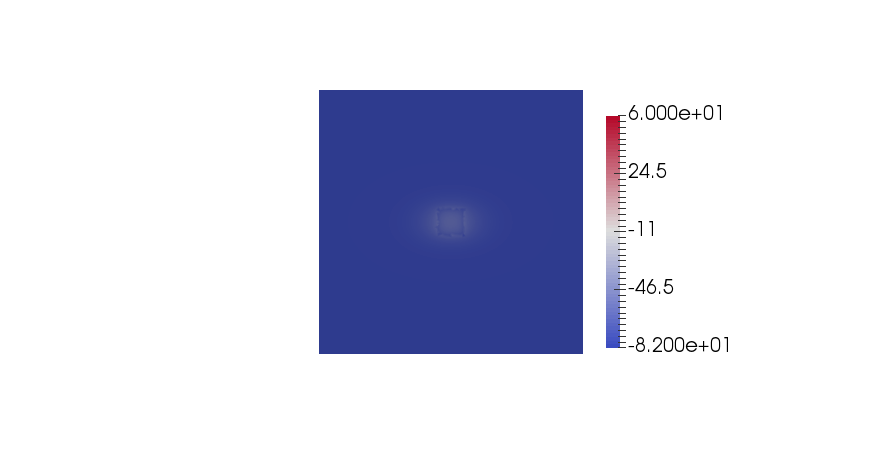
\includegraphics[trim=11cm 0cm 2cm 0cm, clip=true, width=0.9\linewidth]{5s}
      \textbf{(c)} 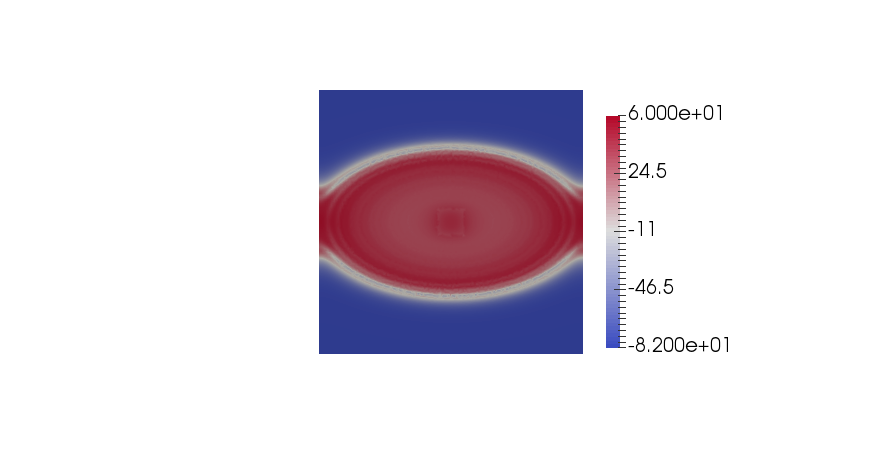
\includegraphics[trim=11cm 0cm 2cm 0cm, clip=true, width=0.9\linewidth]{25s}
    \end{minipage}
    \begin{minipage}{0.47\textwidth}
  \textbf{(b)} 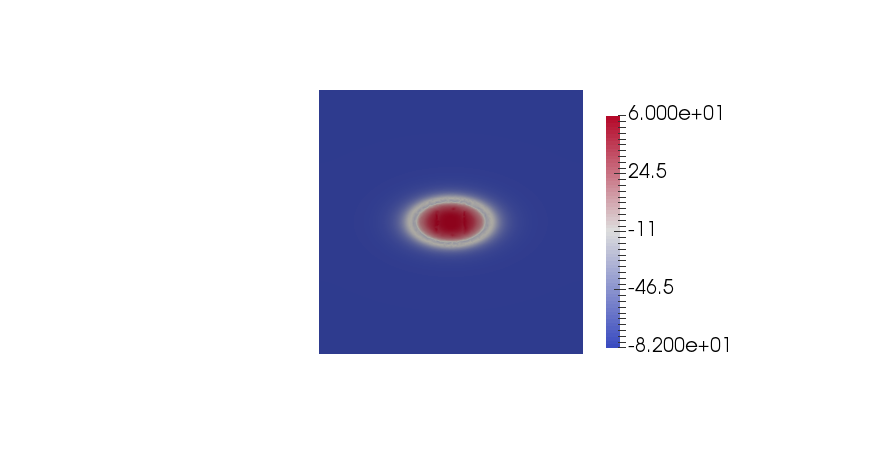
\includegraphics[trim=11cm 0cm 2cm 0cm, clip=true, width=0.9\linewidth]{15s}
  \textbf{(d)} 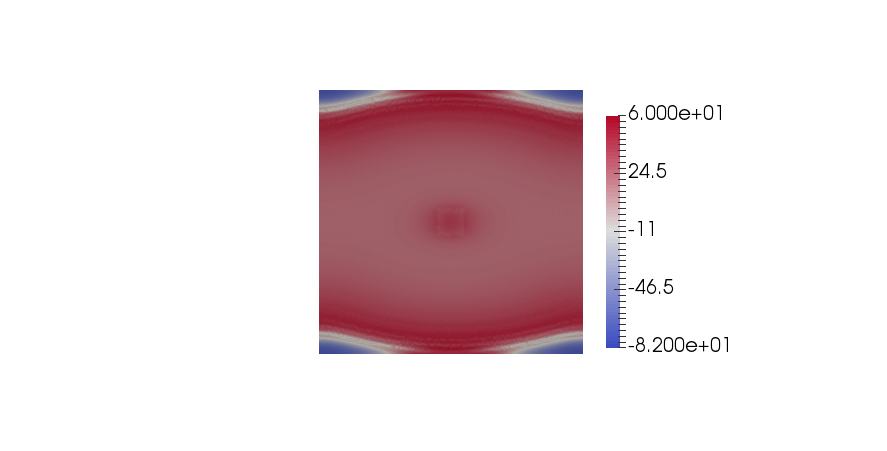
\includegraphics[trim=11cm 0cm 2cm 0cm, clip=true, width=0.9\linewidth]{35s}
    \end{minipage}
    \caption{Heat maps of $u$ of our basic test case at \textbf{(a)} $t=5$ms, \textbf{(b)} $t=15$ms, \textbf{(c)} $t=25$ms and \textbf{(d)} $t=35$ms.}
    \label{fig:1}
\end{figure}
%trim={<left> <lower> <right> <upper>}
\section{The inverse problem} \label{The inverse problem}
It is possible to obtain measurements $u_{\text{obs}}$ of the transmembrane potential and measurements $c_{\text{obs}}$ of the intracellular calcium concentration $c$ over the whole domain $H$ at discrete points in time, where the calcium concentration $c$ is one of the 38 state variables $\mathbf{s}$ of the Grandi cell model. With those measurements, we can estimate the value of the parameters in our model, using an adjoint-based approach.\footnote{See, for example, \cite{Gunzburger} for an introductory text in adjoint-based optimization methods.} Here, as an example, we will try to estimate the values of the $GNa$ parameter from the Grandi cell model.
We can formulate this problem as an optimisation problem: find $GNa$, such that the functional
\begin{eqnarray}
\mathcal{J}(v, c, GNa)= \frac{1}{N} \sum_{i=1}^{N} ||v-v_{\text{obs}}(t_i)||^2_{L^2(H)} + ||c-c_{\text{obs}}(t_i) ||^2_{L^2(H)},\label{J}
\end{eqnarray}
%\begin{eqnarray} \nonumber
%\mathcal{J}(v, c, GNa)= \\ \frac{1}{N} \sum_{i=1}^{N} \int_{H}(v(\textbf{x},t_i)-\Phi(\textbf{x},t_i))^2 \: \text{d}\textbf{x} + \int_{H}\left(c(\textbf{x},t_i)-\Psi(\textbf{x},t_i)\right)^2 \: \text{d}\textbf{x},\label{J}
%\end{eqnarray}
is minimized, subject to the requirements that $v, c$ and $GNa$ satisfy the state system of equations \eqref{eq:a}-\eqref{eq:c} and initial conditions $v(\textbf{x},0)=v_0(\textbf{x})$ and $\mathbf{s}(\mathbf{x},0)=\mathbf{s}_0(\mathbf{x})$. Here, $N$ are the number of measurements in time and $t_i$, $i=1, \dots N$ the respective moments in time.
% https://fenicsproject.org/qa/6675/hdf-file-read-write-for-time-series
To find a minimum for our functional $\mathcal{J}$, we will need to determine its total derivative with respect to the optimization parameter $Gna$. We use the 
%\begin{eqnarray}
%\frac{\text{D}\mathcal{J}}{\text{D}{Gna}}=\frac{\partial \mathcal{J}}{\partial v}\frac{\partial v}{\partial Gna}
%\frac{\text{D}\mathcal{J}}{\text{D}{M_1}}=\frac{\partial \mathcal{J}}{\partial v}\frac{\partial v}{\partial M_1}+\frac{\partial \mathcal{J}}{\partial M_1}
%=\int_0^T\int_{\tilde{H}}(v-\Phi)\frac{\partial v}{\partial M_1} \: \text{d}\textbf{x}\text{dt}  + \frac{\alpha}{2}\frac{\partial\mathcal{R}}{\partial M_1} \\
%\frac{\text{D}\mathcal{J}}{\text{D}{M_2}}=\frac{\partial \mathcal{J}}{\partial v}\frac{\partial v}{\partial M_2}+\frac{\partial \mathcal{J}}{\partial M_2}
%=\int_0^T\int_{\tilde{H}}(v-\Phi)\frac{\partial v}{\partial M_2} \: \text{d}\textbf{x}\text{dt}  + \frac{\alpha}{2}\frac{\partial\mathcal{R}}{\partial M_2}. \label{totdef}
%\end{eqnarray}

%We will use an adjoint-based approach.\footnote{See, for example, \cite{Gunzburger} for an introductory text in adjoint-based optimization methods. See \cite{Yang} for an adjoint-based approach for the estimation of the cardiac conductivity paramters of the bidomain equations.} Consider the Lagrangian functional:
%\begin{eqnarray} 
%% L
%\mathcal{L}(v, \mathbf{M}, \mathbf{s}, \lambda, \boldsymbol{\mu})=
%% J
%\mathcal{J}(v, \mathbf{M}) 
%\nonumber \\
%% \lambda
%-\int_0^T\int_{H} \lambda \left(\frac{\partial v}{\partial t} + I_{ion}(v,\mathbf{s}) -\nabla \cdot(\mathbf{M}\nabla v) - I_s)\right) \:\text{d}\textbf{x}\text{dt} 
%\nonumber \\
%% mu
%-\int_0^T \int_{H} \boldsymbol{\mu} \cdot \left(\frac{\partial \mathbf{s}}{\partial t}- \mathbf{F}(\mathbf{s},v)\right) \:\text{d}\textbf{x}\text{dt}.
%\end{eqnarray}
%Setting the first variation with respect to the state variables $v$ and $\mathbf{s}$ equal to zero yields the adjoint system:
%\begin{eqnarray} \label{ad1}
%\frac{\partial \lambda}{\partial t} + \lambda \frac{\partial I_{ion}}{\partial v} -\nabla \cdot(\mathbf{M}\nabla \lambda) + \boldsymbol{\mu} \cdot \frac{\partial \mathbf{F}}{\partial v}
% = v-\Phi \qquad &\text{on}& \qquad \tilde{H}, \\\label{ad2}
%\frac{\partial \lambda}{\partial t} + \lambda \frac{\partial I_{ion}}{\partial v} -\nabla \cdot(\mathbf{M}\nabla \lambda) + \boldsymbol{\mu} \cdot \frac{\partial \mathbf{F}}{\partial v} = 0 \qquad &\text{on}& \qquad H-\tilde{H}, \\\label{ad3}
%\lambda\frac{\partial I_{ion}}{\partial \mathbf{s}} + 
%\frac{\partial\boldsymbol{\mu}}{\partial{dt}}-\boldsymbol{\mu}\cdot \frac{\partial\mathbf{F}}{\partial \mathbf{s}} = 0\qquad &\text{on}& \qquad H,
%\end{eqnarray}
%with terminal conditions $\lambda(\textbf{x},T)=0$ and $\boldsymbol{\mu}(\mathbf{x},T)=0$. Plugging equations \eqref{ad1}-\eqref{ad2} into equation \eqref{totdef} yields:
%\begin{eqnarray}
%\frac{\text{D}\mathcal{J}}{\text{D}\mathbf{M}}
%=\int_0^T\int_{{H}}\left(\frac{\partial \lambda}{\partial t} + \lambda \frac{\partial I_{ion}}{\partial v} -\nabla \cdot(\mathbf{M}\nabla \lambda) + \boldsymbol{\mu} \cdot \frac{\partial \mathbf{F}}{\partial v}\right)\frac{\partial v}{\partial\mathbf{M}} \: \text{d}\textbf{x}\text{dt} + \frac{\alpha}{2}\frac{\partial\mathcal{R}}{\partial \mathbf{M}}. 
%\end{eqnarray}
%We integrate by parts:
%\begin{eqnarray} \nonumber
%\frac{\text{D}\mathcal{J}}{\text{D}\sigma}
%=\int_0^T\int_{{H_i}}\nabla \cdot \sigma_i \nabla \left(\frac{\partial u_i}{\partial\sigma}\right)\xi \: \text{d}\textbf{x}\text{dt}  +\int_0^T\int_{{H_e}}\nabla \cdot \sigma_e \nabla \left(\frac{\partial u_e}{\partial\sigma}\right)\mu \: \text{d}\textbf{x}\text{dt} \\ \nonumber
%+ \int_0^T\int_{{\Gamma}} \left(\frac{\partial u_i}{\partial\sigma}\right)n_i \cdot \sigma_i \nabla \xi + \left(\frac{\partial u_e}{\partial\sigma}\right)n_e \cdot \sigma_e \nabla \mu 
%\: \text{d}\textbf{s}\text{dt} \\ \nonumber
%-\int_0^T\int_{{\Gamma}}
% \xi \left(n_i \cdot \sigma_i \nabla \left(\frac{\partial u_i}{\partial\sigma}\right)\right) + \mu \left(n_e \cdot \sigma_e \nabla \left(\frac{\partial u_e}{\partial\sigma}\right)\right) \: \text{d}\textbf{s}\text{dt} \\
%+ \int_0^T\int_{{\Gamma}}\left(\theta -C_m \frac{\partial \rho}{\partial t} +\rho \frac{\partial{f}}{\partial u_m}-\boldsymbol{\tau}\cdot \frac{\partial\mathbf{g}}{\partial u_m}\right)\frac{\partial u_m}{\partial\sigma} \: \text{d}\textbf{s}\text{dt} + \frac{\alpha}{2}\frac{\partial\mathcal{R}}{\partial \sigma}. 
%\end{eqnarray}
%Now, we differentiate our state equation system \eqref{3}-\eqref{7b} with respect to $\sigma_i$ and $\sigma_e$:
%\begin{eqnarray}
%\frac{\partial}{\partial}
%\end{eqnarray}
%\begin{color}{red} \end{color}
%\section*{Appendix A}
%To derive the adjoint system as given by equations \eqref{ad1}-\eqref{adz}, with terminal conditions $\rho(\textbf{s},T)=0$ and $\boldsymbol{r}(\mathbf{s},T)=0$, we set the first variation of the Lagrangian with respect to the state parameters $u_i, u_e, u_m, I_m$ and $\mathbf{w}$ equal to zero and integrate by parts. Setting the first variation with respect to $u_i$ equal to zero gives us:
%\begin{eqnarray} \nonumber
%\int_0^T \int_{\tilde{H_i}}\tilde{u}_i(u_i-\Phi_i)\: \text{d}\textbf{x}\text{dt} = \\
%\int_0^T \int_{H_i}\xi(\nabla \cdot \sigma_i \nabla \tilde{u}_i)\: \text{d}\textbf{x}\text{dt} +  \int_0^T \int_{\Gamma}-\theta \tilde{u}_i + (\zeta + \eta)(n_i \cdot \sigma_i \nabla \tilde{u}_i)\: \text{d}\textbf{s}\text{dt},
%\end{eqnarray}
%for arbitrary variations $\tilde{u}_i$ of $u_i$.
%We integrate by parts:
%\begin{eqnarray} \nonumber
%\int_0^T \int_{\tilde{H_i}}\tilde{u}_i(u_i-\Phi_i)\: \text{d}\textbf{x}\text{dt} = \int_0^T \int_{H_i}\tilde{u}_i(\nabla \cdot \sigma_i \nabla \xi)\: \text{d}\textbf{x}\text{dt} \\ 
%+  \int_0^T \int_{\Gamma}-\theta \tilde{u}_i + (\zeta + \eta +\xi)(n_i \cdot \sigma_i \nabla \tilde{u}_i) - \tilde{u}_i (n_i \cdot \sigma_i \nabla \xi)\: \text{d}\textbf{s}\text{dt}.
%\end{eqnarray}
%Since variations in $\tilde{u}_i$ are arbitrary, we obtain:
%\begin{eqnarray}
%\nabla \cdot \sigma_i \nabla \xi = u_i-\Phi_i \qquad &\text{on}& \qquad \tilde{H_i}, \\
%\nabla \cdot \sigma_i \nabla \xi = 0 \qquad &\text{on}& \qquad H-\tilde{H_i}, \\
%\zeta+\eta+\xi=0 \qquad &\text{on}& \qquad {\Gamma}, \\
%\theta=-n_i \cdot \sigma_i \nabla \xi \qquad &\text{on}& \qquad {\Gamma}.
%\end{eqnarray}
%Similarly, setting the first variation with respect to$u_e$ equal to zero gives us:
%\begin{eqnarray} \nonumber
%\int_0^T \int_{\tilde{H_e}}\tilde{u}_e(u_e-\Phi_e)\: \text{d}\textbf{x}\text{dt} =
%\int_0^T \int_{H_e}\mu(\nabla \cdot \sigma_e \nabla \tilde{u}_e)\: \text{d}\textbf{x}\text{dt} \\
%+\int_0^T \int_{\delta H_e}\tilde{u_e}\nu\: \text{d}\textbf{s}\text{dt}+  \int_0^T \int_{\Gamma}\theta \tilde{u}_e + \zeta(n_e \cdot \sigma_e \nabla \tilde{u}_e)\: \text{d}\textbf{s}\text{dt},
%\end{eqnarray}
%for arbitrary variations $\tilde{u}_e$ of $u_e$.
%We integrate by parts:
%\begin{eqnarray} \nonumber
%\int_0^T \int_{\tilde{H}}\tilde{u}_e(u_e-\Phi_e)\: \text{d}\textbf{x}\text{dt} = \int_0^T \int_{H_e}\tilde{u}_e(\nabla \cdot \sigma_e \nabla \mu)\: \text{d}\textbf{x}\text{dt} \\ \nonumber +\int_0^T \int_{\deltaH_e} \mu(n_e \cdot \sigma_e \nabla \tilde{u}_e) + \tilde{u}_e (\nu - n_e \cdot \sigma_e \nabla \mu)\: \text{d}\textbf{s}\text{dt} \\
%+  \int_0^T \int_{\Gamma}\theta \tilde{u}_e + (\zeta +\mu)(n_e \cdot \sigma_e \nabla \tilde{u}_e) - \tilde{u}_e (n_e \cdot \sigma_e \nabla \mu)\: \text{d}\textbf{s}\text{dt}.
%\end{eqnarray}
%Since variations in $\tilde{u}_e$ are arbitrary, we obtain:
%\begin{eqnarray}
%\nabla \cdot \sigma_e \nabla \mu = u_e-\Phi_e \qquad &\text{on}& \qquad \tilde{H_e}, \\
%\nabla \cdot \sigma_e \nabla \mu = 0 \qquad &\text{on}& \qquad H-\tilde{H_e}, \\
%\zeta+\mu=0 \qquad &\text{on}& \qquad {\Gamma}, \\
%\theta=n_e \cdot \sigma_e \nabla \mu \qquad &\text{on}& \qquad {\Gamma} \\
%\nu=n_e \cdot \sigma_e \nabla \mu \qquad &\text{on}& \qquad {\delta H}\\
%\mu=0 \qquad &\text{on}& \qquad {\delta H}.
%\end{eqnarray}
%Setting the first variation with respect to $u_m$ equal to zero is equivalent to:
%\begin{eqnarray} \nonumber
%\int_0^T \int_{\tilde{\Gamma}}\tilde{u}_m(u_m-\Phi_m)\: \text{d}\textbf{s}\text{dt} = \\ \nonumber
%\int_0^T \int_{\Gamma}\tilde{u}_m \theta + \rho\left(C_m \frac{\partial \tilde{u}_m}{\partial t} + \frac{\partial f}{\partial {u}_m}\tilde{u}_m\right)-\boldsymbol{\tau}\cdot \frac{\partial\mathbf{g}}{\partial {u}_m}\tilde{u}_m \: \text{d}\textbf{s}\text{dt}\\
%+\int_\Gamma \tilde{u}_m(\mathbf{s},0)\kappa(\mathbf{s},0) \: \text{d}\textbf{s},
%\end{eqnarray}
%for arbitrary variations $\tilde{u}_m$ of $u_m$.
%We integrate by parts:
%\begin{eqnarray} \nonumber
%\int_0^T \int_{\tilde{\Gamma}}\tilde{u}_m(u_m-\Phi_m)\: \text{d}\textbf{s}\text{dt} = \\ \nonumber
%\int_0^T \int_{\Gamma} \tilde{u}_m \theta- \tilde{u}_m C_m \frac{\partial \rho}{\partial t} + \rho\frac{\partial{f}}{\partial {u}_m}\tilde{u}_m-\boldsymbol{\tau}\cdot \frac{\partial\mathbf{g}}{\partial {u}_m}\tilde{u}_m \: \text{d}\textbf{s}\text{dt} \\ +\int_\Gamma \tilde{u}_m(\mathbf{s},0)\kappa(\mathbf{s},0) + C_m \left(\rho(\mathbf{s},T) \tilde{u}_m(\mathbf{s},T)- \rho(\mathbf{s},0) \tilde{u}_m(\mathbf{s},0)
%\right)\: \text{d}\textbf{s}.
%\end{eqnarray}
%Since variations in $\tilde{u}_m$ are arbitrary, we obtain:
%\begin{eqnarray} \nonumber
%\theta - C_m \frac{\partial \rho}{\partial t} +\rho \frac{\partial{f}}{\partial u_m}-\boldsymbol{\tau}\cdot \frac{\partial\mathbf{g}}{\partial u_m}= u_m-\Phi_m \qquad &\text{on}& \qquad \tilde{\Gamma}, \\
%\theta - C_m \frac{\partial \rho}{\partial t} +\rho \frac{\partial{f}}{\partial u_m}-\boldsymbol{\tau}\cdot \frac{\partial\mathbf{g}}{\partial u_m}= 0 \qquad &\text{on}& \qquad \Gamma-\tilde{\Gamma},
%\end{eqnarray}
%$C_m\rho(\textbf{s},0)=\kappa(\textbf{s},0)$ and $\rho(\textbf{s},T)=0$.
%Setting the first variation with respect to $I_m$ equal to zero is equivalent to:
%\begin{eqnarray} 
%\int_0^T \int_{\tilde{\Gamma}}(\eta+\rho)\tilde{I}_m\: \text{d}\textbf{s}\text{dt} = 0,
%\end{eqnarray}
%for arbitrary variations $\tilde{I}_m$ of $I_m$. Since variations in $\tilde{I}_m$ are arbitrary, we obtain:
%\begin{eqnarray}
%\eta=-\rho \qquad &\text{on}& \qquad \tilde{\Gamma}.
%\end{eqnarray}
%Finally, setting the first variation with respect to $\mathbf{w}$ equal to zero gives us:
%\begin{eqnarray} 
%\int_0^T \int_{{\Gamma}}\rho\frac{\partial f}{\partial \mathbf{w}}\tilde{\mathbf{w}} + \boldsymbol{\tau} \cdot \left( \frac{\text{d}\mathbf{\tilde{w}}}{\text{dt}}- \frac{\partial \mathbf{g}}{\partial \mathbf{w}}\tilde{\mathbf{w}}\right)\: \text{d}\textbf{x}\text{dt} + \int_{{\Gamma}}\boldsymbol{\lambda}(\mathbf{s},0)\cdot \mathbf{\tilde{w}(\mathbf{s},0)}\: \text{d}\textbf{x}= 0,
%\end{eqnarray}
%for arbitrary variations $\tilde{\mathbf{w}}$ of $\mathbf{w}$.
%We integrate by parts:
%\begin{eqnarray} \nonumber
%\int_0^T \int_{{\Gamma}}\rho\frac{\partial f}{\partial \mathbf{w}}\tilde{\mathbf{w}} - \mathbf{\tilde{w}} \cdot \frac{\text{d}\boldsymbol{\tau}}{\text{dt}}- \boldsymbol{\tau} \cdot\frac{\partial \mathbf{g}}{\partial \mathbf{w}}\tilde{\mathbf{w}}\: \text{d}\textbf{x}\text{dt} \\ +\int_{{\Gamma}}\boldsymbol{\tau}(\mathbf{s},T)\cdot\mathbf{\tilde{w}}(\mathbf{s},T) - \boldsymbol{\tau}(\mathbf{s},0)\cdot\mathbf{\tilde{w}}(\mathbf{s},0)+ \boldsymbol{\lambda}(\mathbf{s},0)\cdot \mathbf{\tilde{w}(\mathbf{s},0)}\: \text{d}\textbf{x}= 0.
%\end{eqnarray}
%Since variations in $\tilde{\mathbf{w}}$ are arbitrary, we obtain:
%\begin{eqnarray}
%\frac{\text{d}\boldsymbol{\tau}}{\text{dt}}-\rho \frac{\partial{f}}{\partial \mathbf{w}}+\boldsymbol{\tau}\cdot \frac{\partial\mathbf{g}}{\partial \mathbf{w}} = 0\qquad &\text{on}& \qquad \Gamma,
%\end{eqnarray}
%$\boldsymbol{\tau}(\textbf{s},0)=\boldsymbol{\lambda}(\textbf{s},0)$ and $\boldsymbol{\tau}(\textbf{s},T)=0$.

\begin{thebibliography}{99}
\bibitem{Grandi} Grandi, Pasqualini, Puglisi, \& Bers. (2009). A Novel Computational Model of the Human Ventricular Action Potential and Ca transient. \textit{Biophysical Journal, 96}(3), 664a-665a.
\bibitem{Gunzburger} Gunzburger, M. (2003). \textit{Perspectives in flow control and optimization} (Advances in design and control). Philadelphia, Pa.: SIAM.
\bibitem{Sundnes} Sundnes, J., Nielsen, B., Mardal, K., Cai, X., Lines, G., \& Tveito, A. (2006). On the Computational Complexity of the Bidomain and the Monodomain Models of Electrophysiology. \textit{Annals of Biomedical Engineering, 34}(7), 1088-1097.
%\bibitem{Yang} Yang, H., \& Veneziani, A. (2015). Estimation of cardiac conductivities in ventricular tissue by a variational approach. \textit{Inverse Problems, 31}(11), 115001.
\end{thebibliography}
\end{document}